\chapter{Diagram E--pH}\label{ch:b1:e-ph-diagrams}

Paku besi yang dibiarkan di dalam air hujan berkarat; paku yang sama di
dalam larutan yang sangat basa tetap mengilap selama berminggu-minggu.
Lambung baja sebuah kapal membawa bongkah-bongkah seng yang larut
menggantikannya, dan atap tembaga berubah hijau tetapi tidak pernah
lenyap. \omterm{def:b1:nernst:couple}{Pasangan redoks} yang potensialnya bergantung pada pH, pengendapan
hidroksida dan oksida, kesetimbangan asam--basa: ketiganya bekerja
sekaligus, dan satu peta menghimpun semuanya. Pada grafik potensial
terhadap pH, setiap spesies sebuah unsur mendapat daerah tempat spesies
itu menjadi bentuk yang stabil; membaca peta itu menunjukkan spesies mana
yang bertahan di dalam air, mana yang saling bereaksi, dan di mana
sebuah logam terkorosi.

\begin{recall}
\omterm{thm:b1:nernst:nernst}{Persamaan Nernst}, \omterm{def:b1:nernst:electrode-potential}{potensial standar}, dan peramalan reaksi redoks terdapat
pada \cref{ch:b1:nernst}; \omterm{def:b1:predominant-reaction:predominance}{diagram predominansi} pada
\cref{ch:b1:predominant-reaction}; ambang pengendapan hidroksida dan
\omterm{def:b1:precipitation:existence-domain}{daerah keberadaan} padatan pada \cref{ch:b1:precipitation}. Semua
potensial pada \qty{25}{\celsius}, dengan $RT\ln 10/F = \qty{0.059}{V}$.
\end{recall}

\begin{omfigure}
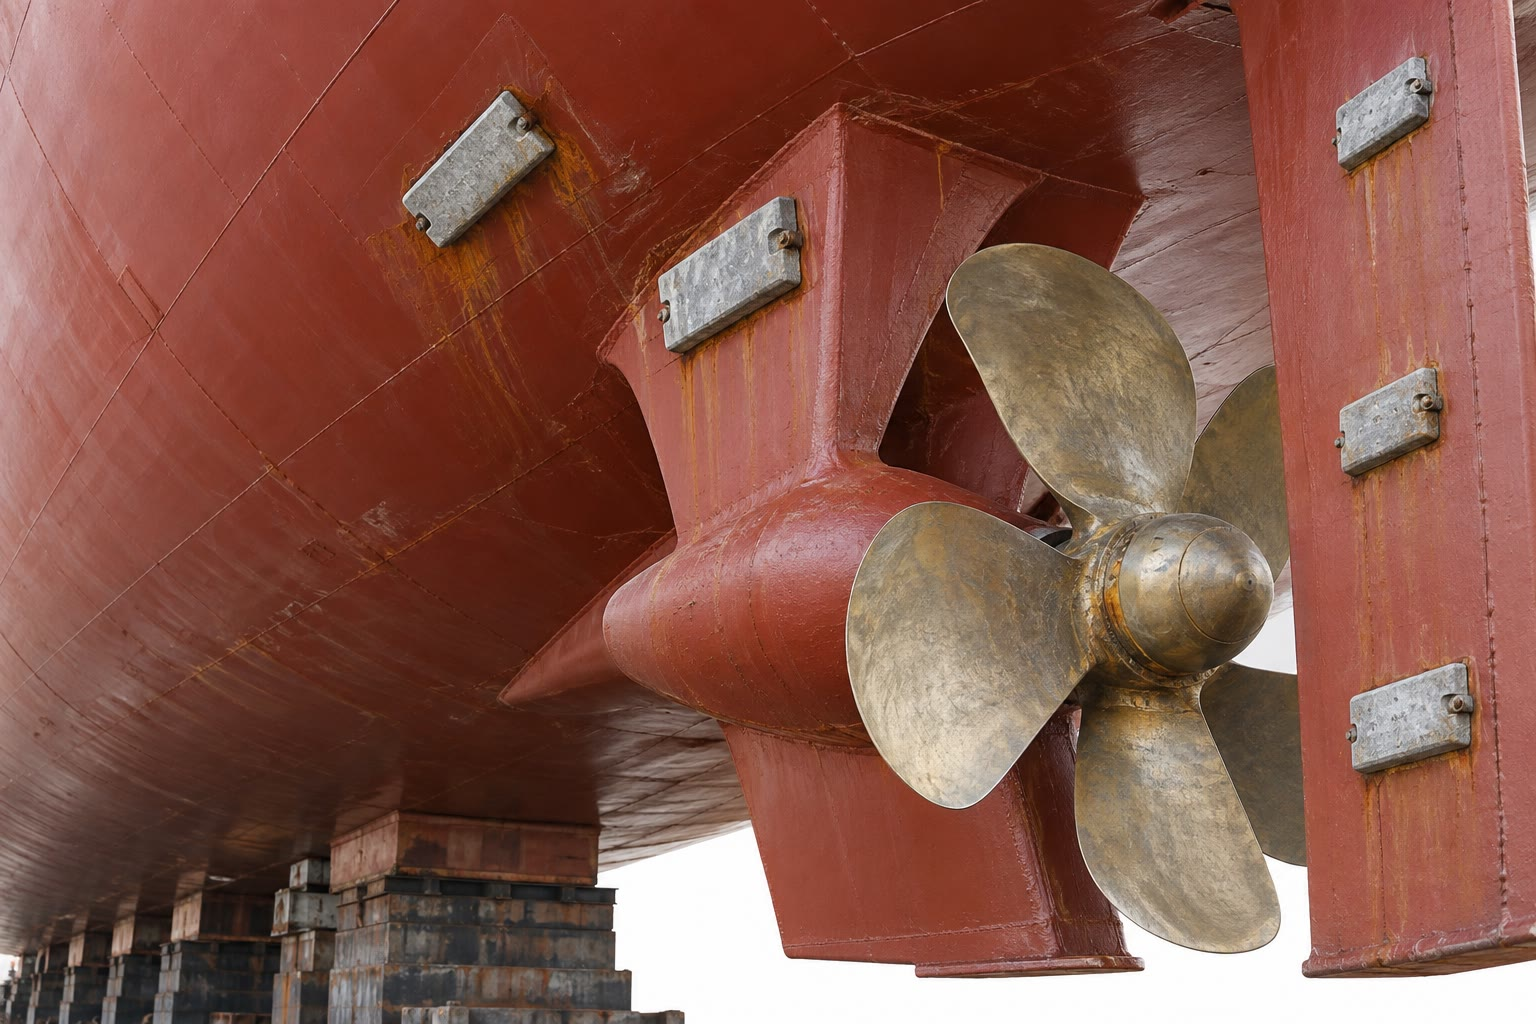
\includegraphics[width=0.6\linewidth]{images/book2/ai/b1-14-ship-anodes.jpg}

{\small Buritan sebuah kapal di dok kering. Bongkah-bongkah abu-abu yang
dipasang pada lambung di dekat baling-baling adalah seng: di dalam air
laut bongkah itu terkorosi menggantikan baja
(\cref{exo:b1:e-ph-diagrams:12}).}
\end{omfigure}

\section{Konvensi}

\begin{definition}[Diagram potensial--pH, konsentrasi kerja]\label{def:b1:e-ph-diagrams:e-ph-diagram}
\emph{Diagram potensial--pH}\index{diagram potensial--pH} sebuah unsur
adalah bidang $(\mathrm{pH}, E)$ yang dibagi menjadi daerah-daerah, yang
masing-masing merupakan daerah predominansi (spesies terlarut) atau
\omterm{def:b1:precipitation:existence-domain}{daerah keberadaan} (padatan) satu bentuk unsur itu. Diagram itu digambar
untuk \emph{konsentrasi kerja}\index{konsentrasi kerja} $c$ yang dipilih,
yaitu konsentrasi total unsur itu dalam larutan, dengan konvensi-konvensi
berikut:
\begin{itemize}
  \item pada batas antara dua spesies terlarut, masing-masing berada pada
        $c$ (dihitung dalam atom unsur itu);
  \item pada batas antara spesies terlarut dan padatan, spesies terlarut
        berada pada $c$ dan padatannya baru saja ada;
  \item gas-gas berada pada \qty{1}{bar}.
\end{itemize}
Dalam bab ini $c = \qty{0.010}{mol/L}$.
\end{definition}

Bentuk-bentuk unsur itu diurutkan menurut \omterm{def:b1:nernst:oxidation-number}{bilangan oksidasinya}: makin
tinggi bilangannya, makin tinggi letaknya pada diagram (bentuk
teroksidasi stabil pada potensial tinggi). Pada \omterm{def:b1:nernst:oxidation-number}{bilangan oksidasi} yang
sama, bentuk-bentuk yang lebih basa (hidroksida, oksida, \omterm{def:b1:complexation:complex}{kompleks}
hidrokso) berada di sebelah kanan.

\begin{proposition}[Kemiringan sebuah batas]\label{prop:b1:e-ph-diagrams:boundary-slope}
Batas antara dua spesies dengan \omterm{def:b1:nernst:oxidation-number}{bilangan oksidasi} yang berbeda, yang
\omterm{def:b1:nernst:couple}{setengah reaksinya} mempertukarkan $n$ elektron dan $m$ proton,
$\mathrm{Ox} + m\,\ce{H+} + n\,\mathrm{e^-} \rightleftharpoons \mathrm{Red} +
\cdots$, adalah garis lurus dengan kemiringan $-0.059\,m/n$ volt per
satuan pH. Batas antara dua spesies dengan \omterm{def:b1:nernst:oxidation-number}{bilangan oksidasi} yang sama
berupa garis tegak.
\end{proposition}

\begin{proof}
\omterm{thm:b1:nernst:nernst}{Persamaan Nernst} memberikan $E = E^\circ + \frac{0.059}{n}\log\frac{[\mathrm{Ox}]
[\ce{H+}]^m}{[\mathrm{Red}]} = E^\circ + \frac{0.059}{n}\log\frac{[\mathrm{Ox}]}
{[\mathrm{Red}]} - \frac{0.059\,m}{n}\,\mathrm{pH}$, dan pada batas itu
konsentrasi-konsentrasinya ditetapkan oleh konvensi. Dua spesies dengan
\omterm{def:b1:nernst:oxidation-number}{bilangan oksidasi} yang sama dihubungkan oleh kesetimbangan asam--basa
atau pengendapan tanpa elektron, yang tetapannya menetapkan pH batas itu
berapa pun potensialnya.
\end{proof}

\section{Air}

\begin{proposition}[Kedua garis air]\label{prop:b1:e-ph-diagrams:water-lines}
Pada gas \qty{1}{bar}, air tereduksi menjadi hidrogen di bawah garis
$E = -0.059\,\mathrm{pH}$ dan teroksidasi menjadi oksigen di atas garis
$E = 1.23
- 0.059\,\mathrm{pH}$.
\end{proposition}

\begin{proof}
\ce{2H+ + 2e- -> H2}: $E = 0 + \frac{0.059}{2}\log\frac{[\ce{H+}]^2}{p(\ce{H2})}
= -0.059\,\mathrm{pH}$ pada $p = 1$. \ce{O2 + 4H+ + 4e- -> 2H2O}: $E = 1.23 +
\frac{0.059}{4}\log(p(\ce{O2})[\ce{H+}]^4) = 1.23 - 0.059\,\mathrm{pH}$. Di
bawah garis pertama \ce{H2} adalah bentuk stabil pasangan itu (air
tereduksi); di atas garis kedua, \ce{O2}.
\end{proof}

\begin{definition}[Daerah kestabilan air]\label{def:b1:e-ph-diagrams:water-domain}
Pita di antara kedua garis itu, selebar \qty{1.23}{V} pada setiap pH,
adalah \emph{daerah kestabilan air}\index{daerah kestabilan air}: spesies
yang daerahnya seluruhnya berada di dalamnya tidak mengoksidasi maupun
mereduksi air.
\end{definition}

\section{Menyusun sebuah diagram: besi}

\begin{method}[Menyusun diagram potensial--pH]\label{met:b1:e-ph-diagrams:build}
\begin{enumerate}
  \item Daftarkan spesies-spesiesnya dan urutkan menurut \omterm{def:b1:nernst:oxidation-number}{bilangan
        oksidasi}: untuk besi, \ce{Fe} (0), \ce{Fe^2+} dan \ce{Fe(OH)2}
        ($+$II), \ce{Fe^3+} dan \ce{Fe(OH)3} ($+$III).
  \item Pada setiap \omterm{def:b1:nernst:oxidation-number}{bilangan oksidasi}, tentukan batas-batas tegak dari
        kesetimbangan pengendapan (atau asam--basa) pada \omterm{def:b1:e-ph-diagrams:e-ph-diagram}{konsentrasi kerja}
        (\cref{ch:b1:precipitation}).
  \item Untuk setiap pasangan \omterm{def:b1:nernst:oxidation-number}{bilangan oksidasi} yang bertetangga, tuliskan
        \omterm{def:b1:nernst:couple}{setengah reaksi} pada setiap rentang pH beserta \omterm{thm:b1:nernst:nernst}{persamaan Nernst-nya}
        dengan konvensi itu; hasilnya sebuah batas lurus dengan kemiringan
        yang diketahui.
  \item Rangkaikan garis-garis itu dari kiri ke kanan; di tempat tiga
        garis bertemu, setiap garis hanya berlanjut pada sisi tempat kedua
        spesiesnya sama-sama stabil.
  \item Periksalah: daerah-daerahnya tidak boleh bertumpang tindih, dan
        kemiringannya harus sesuai dengan
        \cref{prop:b1:e-ph-diagrams:boundary-slope}.
\end{enumerate}
\end{method}

\begin{example}[Batas-batas besi]\label{ex:b1:e-ph-diagrams:iron}
Dengan $c = \qty{0.010}{mol/L}$ (dan tetapan-tetapan pada \cref{ch:b1:precipitation,ch:b1:nernst}):
\begin{itemize}
  \item \ce{Fe^3+}/\ce{Fe(OH)3}: $\mathrm{pH} = 14.00 - \frac13(38.55 - 2) = 1.82$;
        \ce{Fe^2+}/\ce{Fe(OH)2}: $\mathrm{pH} = 14.00 - \frac12(16.31 - 2) = 6.85$.
  \item \ce{Fe^2+}/\ce{Fe}: $E = -0.41 + 0.030\log c = -0.47$~V (pH di bawah 6.85).
  \item \ce{Fe^3+}/\ce{Fe^2+}: $E = 0.77$~V (keduanya pada $c$, pH di bawah 1.82).
  \item \ce{Fe(OH)3}/\ce{Fe^2+}: \ce{Fe(OH)3 + 3H+ + e- -> Fe^2+ + 3H2O}, kemiringan
        $-0.177$: $E = 1.09 - 0.177\,\mathrm{pH}$ antara pH 1.82 dan 6.85.
  \item \ce{Fe(OH)3}/\ce{Fe(OH)2}: satu elektron, satu proton, $E = 0.28 -
        0.059\,\mathrm{pH}$; \ce{Fe(OH)2}/\ce{Fe}: dua elektron, dua
        proton, $E = -0.07 - 0.059\,\mathrm{pH}$ (pH di atas 6.85).
\end{itemize}
Titik potong sumbunya diperoleh dari kekontinuan di titik-titik rangkap
tiga, atau langsung dari energi Gibbs pembentukan; diagram di bawah
dihitung dengan cara yang kedua, dan batas-batasnya berbeda dari
nilai-nilai bulat ini kurang dari \qty{0.01}{V} atau 0.01 satuan pH.
% ledger: dfg:Fe2+_ao, dfg:Fe3+_ao, dfg:Fe_OH2_cr, dfg:Fe_OH3_cr, dfg:H2O_l, dfg:OH-_ao (boundaries computed in figdata/bachelor-1/eph-diagrams.py)
\end{example}

\begin{omfigure}
\begin{tikzpicture}
\begin{axis}[
  width=0.8\linewidth, height=8.2cm, xmin=0, xmax=14, ymin=-1.2, ymax=1.6,
  axis x line=bottom, axis y line=left, xlabel={pH}, ylabel={$E$ (V)},
  xtick={0,2,4,6,8,10,12,14}, ytick={-1,-0.5,0,0.5,1,1.5},
  unbounded coords=jump, clip=true,
  tick label style={font=\small}, label style={font=\small}]
\addplot[black!45, dashed] table[x=pH, y=H2] {figdata/out/bachelor-1-eph-diagrams-water.dat};
\addplot[black!45, dashed] table[x=pH, y=O2] {figdata/out/bachelor-1-eph-diagrams-water.dat};
\addplot[omDef, very thick] table[x=pH, y=E] {figdata/out/bachelor-1-eph-diagrams-iron.dat};
\node[font=\small] at (axis cs:3.2,-0.85) {\ce{Fe}};
\node[font=\small] at (axis cs:3.4,0.15) {\ce{Fe^2+}};
\node[font=\small] at (axis cs:0.9,1.45) {\ce{Fe^3+}};
\node[font=\small] at (axis cs:8.5,0.25) {\ce{Fe(OH)3}};
\node[font=\scriptsize] at (axis cs:11.0,-0.56) {\ce{Fe(OH)2}};
\node[font=\scriptsize, black!55, rotate=-14, anchor=south] at (axis cs:12.0,0.52) {\ce{O2}/\ce{H2O}};
\node[font=\scriptsize, black!55, rotate=-14, anchor=south] at (axis cs:2.2,-0.11) {\ce{H2O}/\ce{H2}};
\end{axis}
\end{tikzpicture}

{\small \omterm{def:b1:e-ph-diagrams:e-ph-diagram}{Diagram potensial--pH} besi untuk $c = \qty{0.010}{mol/L}$ (garis
utuh), dengan kedua garis air (putus-putus). Setiap batas dihitung dari
energi Gibbs pembentukan dalam tabel.}
\end{omfigure}

\section{Tembaga dan seng}

Metode yang sama menghasilkan diagram tembaga (spesies \ce{Cu}, \ce{Cu+},
\ce{Cu2O} pada $+$I, \ce{Cu^2+}, \ce{CuO} pada $+$II) dan seng (\ce{Zn},
\ce{Zn^2+}, \ce{Zn(OH)2}, \ce{Zn(OH)4^2-}). Untuk tembaga, \ce{CuO}
muncul pada $\mathrm{pH} = 14.00 - \frac12(20.64 - 2) = 4.68$, dan ion
\ce{Cu+}, walaupun tercantum, sama sekali tidak mempunyai daerah: dalam
asam, $E^\circ(\ce{Cu+}/\ce{Cu}) = 0.52$~V terletak di atas
$E^\circ(\ce{Cu^2+}/\ce{Cu+}) = 0.16$~V, sehingga daerah yang semestinya
miliknya dicoret oleh kedua tetangganya
(\cref{sec:b1:e-ph-diagrams:reading}). Untuk seng, hidroksidanya muncul
pada pH 6.81 dan larut kembali sebagai \ce{Zn(OH)4^2-} hanya di atas
13.97 pada konsentrasi ini, sebuah jalur tipis di tepi kanan.

\begin{omfigure}
\begin{tikzpicture}
\begin{axis}[name=cu,
  width=0.47\linewidth, height=7cm, xmin=0, xmax=14, ymin=-1.4, ymax=1.6,
  axis x line=bottom, axis y line=left, xlabel={pH}, ylabel={$E$ (V)},
  xtick={0,4,8,12}, ytick={-1,-0.5,0,0.5,1,1.5},
  unbounded coords=jump, clip=true,
  tick label style={font=\small}, label style={font=\small}]
\addplot[black!45, dashed] table[x=pH, y=H2] {figdata/out/bachelor-1-eph-diagrams-water.dat};
\addplot[black!45, dashed] table[x=pH, y=O2] {figdata/out/bachelor-1-eph-diagrams-water.dat};
\addplot[omDef, very thick] table[x=pH, y=E] {figdata/out/bachelor-1-eph-diagrams-copper.dat};
\node[font=\small] at (axis cs:5,-0.7) {\ce{Cu}};
\node[font=\small] at (axis cs:2,0.7) {\ce{Cu^2+}};
\node[font=\small] at (axis cs:9.5,0.75) {\ce{CuO}};
\node[font=\scriptsize] (cuo) at (axis cs:11.8,-1.05) {\ce{Cu2O}};
\draw[->, black!70] (cuo.north) -- (axis cs:10,-0.035);
\node[font=\small, anchor=north] at (axis cs:7,1.58) {tembaga};
\end{axis}
\begin{axis}[at={(cu.east)}, anchor=west, xshift=1.5cm,
  width=0.47\linewidth, height=7cm, xmin=0, xmax=14, ymin=-1.4, ymax=1.6,
  axis x line=bottom, axis y line=left, xlabel={pH}, ylabel={$E$ (V)},
  xtick={0,4,8,12}, ytick={-1,-0.5,0,0.5,1,1.5},
  unbounded coords=jump, clip=true,
  tick label style={font=\small}, label style={font=\small}]
\addplot[black!45, dashed] table[x=pH, y=H2] {figdata/out/bachelor-1-eph-diagrams-water.dat};
\addplot[black!45, dashed] table[x=pH, y=O2] {figdata/out/bachelor-1-eph-diagrams-water.dat};
\addplot[omDef, very thick] table[x=pH, y=E] {figdata/out/bachelor-1-eph-diagrams-zinc.dat};
\node[font=\small] at (axis cs:3.5,-1.15) {\ce{Zn}};
\node[font=\small] at (axis cs:3.2,0.4) {\ce{Zn^2+}};
\node[font=\small] at (axis cs:10.2,0.4) {\ce{Zn(OH)2}};
\draw[->] (axis cs:12.4,1.15) node[left, font=\scriptsize] {\ce{Zn(OH)4^2-}} -- (axis cs:13.95,1.15);
\node[font=\small, anchor=north] at (axis cs:10.5,1.58) {seng};
\end{axis}
\end{tikzpicture}

{\small \omterm{def:b1:e-ph-diagrams:e-ph-diagram}{Diagram potensial--pH} tembaga dan seng ($c =
\qty{0.010}{mol/L}$), dengan garis-garis air (putus-putus). Daerah logam
tembaga bertumpang tindih dengan daerah air; daerah seng seluruhnya
terletak di bawah garis hidrogen.}
% ledger: dfg:Cu+_ao, dfg:Cu2+_ao, dfg:Cu2O_cr, dfg:CuO_cr, dfg:Zn2+_ao, dfg:Zn_OH2_cr, dfg:Zn_OH42-_ao (boundaries computed in figdata/bachelor-1/eph-diagrams.py)
\end{omfigure}

\section{Membaca sebuah diagram}\label{sec:b1:e-ph-diagrams:reading}

\begin{proposition}[Daerah yang terpisah]\label{prop:b1:e-ph-diagrams:disjoint-domains}
Jika, pada pH tertentu, daerah sebuah \omterm{def:b1:nernst:couple}{oksidator} seluruhnya berada di atas
daerah sebuah \omterm{def:b1:nernst:couple}{reduktor}, tanpa bagian bersama, keduanya bereaksi;
spesies-spesies yang daerahnya berbagi suatu wilayah dapat berdampingan
dalam kesetimbangan.
\end{proposition}

\begin{proof}
Pada pH itu, di atas batasnya pasangan \omterm{def:b1:nernst:couple}{oksidator} mempunyai potensial yang
lebih tinggi daripada potensial mana pun yang dapat dicapai pasangan
\omterm{def:b1:nernst:couple}{reduktor}: menurut \cref{prop:b1:nernst:equilibrium-constant} reaksi di
antara keduanya mempunyai $K > 1$, dan reaksi itu berlangsung sampai
salah satunya habis atau daerah-daerahnya bertemu. Di dalam wilayah
bersama keduanya merupakan bentuk stabil pada potensial yang sama: tidak
ada yang mendorong reaksi.
\end{proof}

Besi dan air: daerah logam besi terletak di bawah garis \ce{H2O}/\ce{H2}
pada setiap pH. Besi mereduksi air, dalam larutan asam dengan pelepasan
hidrogen yang terlihat; dengan oksigen terlarut, besi teroksidasi lebih
cepat lagi. Tembaga: daerahnya bertumpang tindih dengan daerah air,
sehingga tembaga tidak mereduksi air atau asam yang tidak bersifat
\omterm{def:b1:nernst:couple}{oksidator}, tetapi oksigen udara, yang berada di atasnya, mengoksidasinya
perlahan-lahan --- patina hijau pada atap adalah produk lanjutan oksidasi
itu bersama karbon dioksida dan senyawa belerang. Sebuah diagram
menunjukkan apa yang mungkin, bukan seberapa cepat: banyak reaksi yang
diizinkannya berlangsung lambat, sebuah persoalan yang dibahas dalam
jilid Tahun~2.

\begin{definition}[Disproporsionasi, komproporsionasi]\label{def:b1:e-ph-diagrams:disproportionation}
\emph{Disproporsionasi}\index{disproporsionasi} adalah reaksi sebuah
spesies dengan dirinya sendiri, dengan sebagian teroksidasi dan sebagian
lagi tereduksi: \ce{2Cu+ -> Cu^2+ + Cu}. Kebalikannya, dua spesies unsur
yang sama yang menghasilkan satu spesies dengan \omterm{def:b1:nernst:oxidation-number}{bilangan oksidasi} di
antaranya, adalah \emph{komproporsionasi}\index{komproporsionasi}:
\ce{2Fe^3+ + Fe -> 3Fe^2+}.
\end{definition}

\begin{proposition}[Kriteria disproporsionasi]\label{prop:b1:e-ph-diagrams:disproportionation-criterion}
Spesies B dengan \omterm{def:b1:nernst:oxidation-number}{bilangan oksidasi} di antara, dalam pasangan A/B dan
B/C, mengalami \omterm{def:b1:e-ph-diagrams:disproportionation}{disproporsionasi} jika $E(\mathrm{B}/\mathrm{C}) > E(\mathrm{A}/\mathrm{B})$:
spesies itu lalu tidak mempunyai daerah sendiri, dan satu batas A/C
menggantikan keduanya.
\end{proposition}

\begin{proof}
B adalah \omterm{def:b1:nernst:couple}{oksidator} pasangan B/C dan \omterm{def:b1:nernst:couple}{reduktor} pasangan A/B. Jika pasangan
B/C terletak di atas A/B, aturan gamma (\cref{met:b1:nernst:predict-redox})
membuat B (\omterm{def:b1:nernst:couple}{oksidator}, pasangan atas) bereaksi dengan B (\omterm{def:b1:nernst:couple}{reduktor},
pasangan bawah), menghasilkan C dan A. Secara geometris, B hanya akan
stabil di atas $E(\mathrm{B}/\mathrm{C})$
dan di bawah $E(\mathrm{A}/\mathrm{B})$, sebuah himpunan kosong.
\end{proof}

\begin{definition}[Daerah imunitas, korosi, dan pasivasi]\label{def:b1:e-ph-diagrams:corrosion-domains}
Pada diagram sebuah logam, daerah logam itu sendiri adalah \emph{daerah
imunitas}\index{daerah imunitas} logam itu (logam itu tidak dapat
teroksidasi);
daerah-daerah ion terlarutnya membentuk \emph{daerah
korosi}\index{daerah korosi}; daerah-daerah oksida dan hidroksida
padatnya, yang dapat melapisi logam itu, membentuk \emph{daerah
pasivasi}\index{daerah pasivasi}. Apakah sebuah lapisan benar-benar
melindungi logam merupakan persoalan kinetika, yang dibahas dalam jilid
Tahun~2.
\end{definition}

\begin{method}[Membaca sebuah diagram]\label{met:b1:e-ph-diagrams:read}
\begin{enumerate}
  \item Tumpangkan garis-garis air: spesies yang daerahnya berada di luar
        pita air bereaksi dengan air (secara termodinamika).
  \item Untuk dua spesies dari unsur yang berbeda, tumpangkan
        diagram-diagramnya: daerah yang terpisah pada pH yang ditinjau
        berarti terjadi reaksi.
  \item Untuk sebuah logam, tentukan titik (pH, $E$) mediumnya: imunitas,
        korosi, atau pasivasi.
  \item Ingatlah bahwa sebuah diagram digambar untuk satu \omterm{def:b1:e-ph-diagrams:e-ph-diagram}{konsentrasi
        kerja}; batas-batas dengan spesies terlarut bergeser sebesar
        $0.059/n$~V per dekade konsentrasi.
\end{enumerate}
\end{method}

Seng melindungi besi: di dalam air laut (pH sekitar 8) seng dan baja
sebuah lambung kapal saling bersentuhan; seng, yang potensialnya lebih
rendah, teroksidasi lebih dahulu dan elektron-elektron yang dilepaskannya
menjaga besi tetap di dalam atau di dekat \omterm{def:b1:e-ph-diagrams:corrosion-domains}{daerah imunitasnya}. Bongkah
seng itu habis terpakai dan diganti pada setiap kunjungan ke dok kering.

\section{Latihan}

\begin{exercise}[$\star$]\label{exo:b1:e-ph-diagrams:1}
Urutkan menurut \omterm{def:b1:nernst:oxidation-number}{bilangan oksidasi} unsurnya spesies-spesies \ce{Mn},
\ce{Mn^2+}, \ce{MnO2}, \ce{MnO4-}, \ce{Mn(OH)2}, serta \ce{Cl-}, \ce{Cl2},
\ce{HClO}, \ce{ClO-}, \ce{ClO3-}.
\end{exercise}

\begin{exercise}[$\star$]\label{exo:b1:e-ph-diagrams:2}
Tentukan kemiringan batas untuk setiap \omterm{def:b1:nernst:couple}{setengah reaksi} berikut:
\ce{Fe(OH)3 + 3H+ + e- -> Fe^2+ + 3H2O}; \ce{2Cu^2+ + H2O + 2e- -> Cu2O + 2H+};
\ce{MnO4- + 8H+ + 5e- -> Mn^2+ + 4H2O}; \ce{Zn(OH)2 + 2H+ + 2e- -> Zn + 2H2O}.
Mengapa salah satunya mempunyai kemiringan positif?
\end{exercise}

\begin{exercise}[$\star$]\label{exo:b1:e-ph-diagrams:3}
Pada pH berapakah garis-garis air melewati 0~V dan melewati
\qty{0.50}{V}? Berapa lebar \omterm{def:b1:e-ph-diagrams:water-domain}{daerah kestabilan air} pada pH 7?
\end{exercise}

\begin{exercise}[$\star$]\label{exo:b1:e-ph-diagrams:4}
Dengan diagram besi, tentukan bentuk besi yang stabil pada
(pH 1, $E = 1.0$~V), (pH 4, $E = 0$), (pH 10, $E = -0.4$~V), dan
(pH 10, $E = 0.5$~V).
\end{exercise}

\begin{exercise}[$\star\star$]\label{exo:b1:e-ph-diagrams:5}
Hitung ulang batas \ce{Fe^2+}/\ce{Fe} dan garis tegak
\ce{Fe^3+}/\ce{Fe(OH)3} untuk \omterm{def:b1:e-ph-diagrams:e-ph-diagram}{konsentrasi kerja} \qty{1.0e-6}{mol/L},
nilai yang dipakai untuk membahas korosi. Daerah-daerah manakah yang
membesar?
\end{exercise}

\begin{exercise}[$\star\star$]\label{exo:b1:e-ph-diagrams:6}
Turunkan batas \ce{Fe(OH)3}/\ce{Fe^2+}: tuliskan \omterm{def:b1:nernst:couple}{setengah reaksinya},
\omterm{thm:b1:nernst:nernst}{persamaan Nernst-nya}, lalu gunakan kekontinuan pada pH 1.82 untuk
menunjukkan bahwa $E = 1.09 -
0.177\,\mathrm{pH}$.
\end{exercise}

\begin{exercise}[$\star\star$]\label{exo:b1:e-ph-diagrams:7}
Tunjukkan dengan tabel \omterm{def:b1:nernst:electrode-potential}{potensial standar} bahwa \ce{Cu+} mengalami
\omterm{def:b1:e-ph-diagrams:disproportionation}{disproporsionasi} pada pH 0, lalu tentukan potensial satu-satunya batas
\ce{Cu^2+}/\ce{Cu} pada $c = \qty{0.010}{mol/L}$.
\end{exercise}

\begin{exercise}[$\star\star$]\label{exo:b1:e-ph-diagrams:8}
Apakah tembaga larut dalam asam klorida pada pH 0 tanpa udara? dalam asam
nitrat (pasangan \ce{NO3-}/\ce{NO}, $E^\circ = 0.96$~V)? Berikan alasannya
dengan diagram dan potensial-potensialnya.
\end{exercise}

\begin{exercise}[$\star\star$]\label{exo:b1:e-ph-diagrams:9}
Larutan besi(II) yang dibiarkan di udara berubah menjadi kuning
kecokelatan. Jelaskan dengan diagram besi dan garis \ce{O2}/\ce{H2O},
lalu tuliskan reaksinya pada pH 3.
\end{exercise}

\begin{exercise}[$\star\star\star$]\label{exo:b1:e-ph-diagrams:10}
Susunlah diagram seng untuk $c = \qty{0.010}{mol/L}$: hitunglah
batas-batas tegak pada pH 6.81 dan 13.97, batas \ce{Zn^2+}/\ce{Zn}, serta
persamaan \ce{Zn(OH)2}/\ce{Zn} dan \ce{Zn(OH)4^2-}/\ce{Zn}.
\end{exercise}

\begin{exercise}[$\star\star\star$]\label{exo:b1:e-ph-diagrams:11}
Tumpangkan diagram besi dan diagram air, lalu bahaslah nasib sebuah paku
besi di dalam air bebas oksigen pada pH 2, pH 7, dan pH 13. Apa yang
berubah dengan adanya oksigen terlarut?
\end{exercise}

\begin{exercise}[$\star\star\star$]\label{exo:b1:e-ph-diagrams:12}
\omterm{def:b1:nernst:cell}{Anode} korban. Lambung baja di dalam air laut (pH 8) dihubungkan dengan
bongkah seng. Dengan diagram-diagramnya, jelaskan logam mana yang
teroksidasi, tuliskan reaksi-reaksinya dengan oksigen terlarut, dan
nyatakan mengapa magnesium juga akan berhasil sedangkan tembaga akan
memperburuk keadaan.
\end{exercise}

\section{Soal: Pemutih dan Kolam Renang}

\begin{problem}[{Soal akhir pekan --- \omterm{def:b1:nernst:oxidation-number}{bilangan oksidasi} klor, \omterm{def:b1:predominant-reaction:bronsted}{pasangan
asam--basa} HClO/ClO\textsuperscript{$-$}, \omterm{def:b1:e-ph-diagrams:e-ph-diagram}{diagram potensial--pH} klor,
dan pH yang di atasnya klor terlarut mengalami \omterm{def:b1:e-ph-diagrams:disproportionation}{disproporsionasi}}]
\label{pb:b1:e-ph-diagrams:1}
Pemutih adalah larutan basa natrium hipoklorit dan natrium klorida;
kolam renang didisinfeksi oleh asam hipoklorit yang dikandungnya, pada
pH yang dijaga sedikit di atas 7. Mencampur pemutih dengan pembersih
yang asam melepaskan gas klor. Data pada \qty{25}{\celsius}:
$E^\circ(\ce{Cl2(aq)}/\ce{Cl-})
= 1.396$~V,
$E^\circ(\ce{HClO}/\ce{Cl2(aq)}) = 1.594$~V,
$\mathrm{p}K_a(\ce{HClO}/\ce{ClO-}) = 7.55$, $RT\ln 10/F = 0.0592$~V;
\omterm{def:b1:e-ph-diagrams:e-ph-diagram}{konsentrasi kerja} $c = \qty{0.010}{mol/L}$ atom klor.

\medskip
\noindent\textbf{Bagian I --- Spesies-spesiesnya.}
\begin{enumerate}
  \item Tentukan \omterm{def:b1:nernst:oxidation-number}{bilangan oksidasi} klor dalam \ce{Cl-}, \ce{Cl2},
        \ce{HClO}, dan \ce{ClO-}.
  \item Urutkan keempat spesies itu pada sumbu vertikal \omterm{def:b1:nernst:oxidation-number}{bilangan
        oksidasi}.
  \item Dua spesies manakah yang mempunyai \omterm{def:b1:nernst:oxidation-number}{bilangan oksidasi} yang sama?
        Bagaimana hubungan keduanya?
  \item Tuliskan \omterm{def:b1:nernst:couple}{setengah reaksi} \ce{Cl2}/\ce{Cl-}.
  \item Tuliskan \omterm{def:b1:nernst:couple}{setengah reaksi} \ce{HClO}/\ce{Cl2}.
  \item Tuliskan \omterm{def:b1:nernst:couple}{setengah reaksi} \ce{ClO-}/\ce{Cl-} dalam larutan basa.
\end{enumerate}

\medskip
\noindent\textbf{Bagian II --- Asam hipoklorit.}
\begin{enumerate}[resume]
  \item Gambarlah \omterm{def:b1:predominant-reaction:predominance}{diagram predominansi} \ce{HClO} dan \ce{ClO-} terhadap
        pH.
  \item Mengapa batas keduanya pada \omterm{def:b1:e-ph-diagrams:e-ph-diagram}{diagram potensial--pH} berupa garis
        tegak?
  \item Hitunglah fraksi asam hipoklorit pada pH 7.4.
  \item Hal yang sama pada pH 8.0. Asam hipoklorit adalah disinfektan
        yang lebih baik: mengapa pengelola kolam menjaga agar pH tidak
        bergeser naik sampai 8?
  \item Dalam pemutih (pH sekitar 12), bentuk manakah yang ada?
\end{enumerate}

\medskip
\noindent\textbf{Bagian III --- Diagramnya.}
Dengan konvensi bab ini, \ce{Cl2(aq)} berada pada $c/2$ dan \ce{Cl-},
\ce{HClO}, \ce{ClO-} pada $c$ pada sebuah batas.
\begin{enumerate}[resume]
  \item Tunjukkan bahwa batas \ce{Cl2}/\ce{Cl-} terletak pada $E = 1.396 +
        0.0296\log\bigl((c/2)/c^2\bigr) = 1.446$~V, tidak bergantung pada
        pH.
  \item Tunjukkan bahwa batas \ce{HClO}/\ce{Cl2} adalah $E = 1.594 -
        0.0296\log 50 - 0.0592\,\mathrm{pH} \approx 1.544 -
        0.0592\,\mathrm{pH}$.
  \item Tentukan pH tempat kedua garis ini berpotongan.
  \item Di luar pH itu, batasnya adalah \ce{HClO}/\ce{Cl-}. Tuliskan
        \omterm{def:b1:nernst:couple}{setengah reaksinya} dan tunjukkan bahwa kemiringannya $-0.0296$.
  \item Hitunglah $E^\circ(\ce{HClO}/\ce{Cl-})$ dari kedua potensial yang
        diberikan.
  \item Tuliskan batas \ce{ClO-}/\ce{Cl-} di atas pH 7.55; periksalah
        kekontinuannya pada pH 7.55.
  \item Sketsalah diagramnya dari pH 0 sampai 14, dengan garis
        \ce{O2}/\ce{H2O}.
  \item Apakah asam hipoklorit stabil di dalam air, secara termodinamika?
        Mengapa sebuah kolam tetap hanya memerlukan penambahan klor yang
        sedikit setiap hari?
\end{enumerate}

\medskip
\noindent\textbf{Bagian IV --- \omterm{def:b1:e-ph-diagrams:disproportionation}{Disproporsionasi} dan bahaya asam.}
\begin{enumerate}[resume]
  \item Di atas pH pada pertanyaan 14, apa yang terjadi pada klor
        terlarut? Tuliskan reaksinya di dalam air dan di dalam larutan
        basa.
  \item Bagaimana pemutih dibuat dari klor?
  \item Di bawah pH yang sama, tuliskan reaksi antara \ce{HClO} dan
        \ce{Cl-}. Apa nama reaksi itu?
  \item Sebuah pembersih toilet yang asam membawa pemutih ke pH 1. Apa
        yang terjadi?
  \item Mengapa bahayanya lebih kecil dengan produk yang agak asam
        (pH 4)? Jawablah dengan diagram, lalu berikan batasannya.
  \item Nyatakan, sampai satu desimal, pH yang di atasnya klor terlarut
        mengalami \omterm{def:b1:e-ph-diagrams:disproportionation}{disproporsionasi} pada $c = \qty{0.010}{mol/L}$.
\end{enumerate}
\end{problem}
